\documentclass[11pt]{report}
\usepackage{amsmath, amsthm}
\usepackage[pdftex]{graphicx}
\usepackage{psfrag,epsf}
\usepackage{enumerate}
\usepackage{natbib}
\usepackage{float}
\restylefloat{table}

\usepackage{amssymb}
\usepackage{multirow}
\usepackage{float}

\usepackage{Sweave}
\begin{document}
\Sconcordance{concordance:icenReg.tex:icenReg.Rnw:%
1 13 1 1 0 635 1}


\title{Using {\bf{icenReg}} for interval censored data in {\bf{R} } \\ v1.3.0}
\author{Clifford Anderson-Bergman}
\maketitle


\tableofcontents

\chapter{Introduction}

  This manual is meant to provide an introduction to using {\bf icenReg} to 
  analyze interval censored data. It is written with expectation that the reader
  is familiar with basic survival analysis methods. Familiarity with the Kaplan 
  Meier curves and Cox proportional hazards model should be sufficient. 

  \section{Interval Censoring}

  Interval censoring occurs when a response is known only up to an interval. 
  A classic example is testing for diseases at a doctor's clinic; if a 
  subject tests negative at $t_1$ and positive at $t_2$, all that is known is
  that the subject acquired the disease in ($t_1$, $t_2$), rather than an exact time. 
  Other classic examples include examining test mice for tumors after sacrifice 
  (results in \emph{current status} or \emph{case I} interval censored data, in which
  all observations are either left or right censored, as opposed to the more general
  \emph{case II}, which allows for any interval),
  customer choice models in economics (customers are presented a price
  for a product and chose to purchase or not, researcher wants to know distribution of 
  maximum spending amount; this results in current status data again), 
  data reduction methods for sensor analyses (to reduce load on sensor system, message
  is intentionally surpressed if outcome is in an expected region) and data binning 
  (responses reported only up to an interval, in some cases to keep the subjects
  anonymous, in some cases to reduce size of data). 

  
  Often interval censoring is ignored in analysis. For example, age is usually reported only 
  up to the year, rather than as a continuous variable; when a subject reports that their age is 33,
  the information we have is really that their age is in the interval [33,34). 
  In the case that these intervals are very short relative to the question of interest,
  such as with reported age when the scientific quesiton is about age of onset
  of type II diabetes, 
  the bias introduced by ignoring the interval censoring may be 
  small enough to be safely ignored. However, in the case that the width of intervals is 
  non-trivial, statistical methods that account for this should be used for reliable analysis. 
  
  Standard notation for interval censoring is that each observation contains a response
  interval $[l_i,r_i]$ such that the true event time is known to have occurred within. Note
  that this allows for uncensored observations ($l_i = r_i$), right censored 
  ($r_i = \infty$), left censored ($l_i = 0$) or none of the above 
  ($0 < l_i < r_i < \infty$). 
  
  In {\bf icenReg}, the response value is allowed to be interval censored. If our 
  data contains the values \texttt{L} and \texttt{R}, representing the left and 
  right sides of the response interval, we can pass our response to a regression model
  using either
  
  \begin{verbatim}
  cbind(L, R)
  Surv(L, R, type = "interval2")
  \end{verbatim}
  
  It is worth nothing that other R packages, specifically for non-parametric estimation, 
  allow you to declare whether the response intervals are open, closed or a combination
  of partially opened, for example $[l_i, r_i)$. In {\bf icenReg}, it is always assumed 
  that the intervals are closed. 
  
  \section{Classic Estimators}
  
  The topic of interval censoring began in the field of survival analysis. 
  Although it is now considered in other fields of study (such as tobit regression),
  at this time {\bf{icenReg}} focusses on survival models. 
  
  
  One of the earliest models is the Non-Parametric Maximum Likelihood Estimator 
  (NPMLE), also referred to as Turnbull's Estimator. This is a generalization of
  the Kaplan Meier curves (which is a generalization of the empirical distribution function)
  that allows for interval censoring. Unlike the Kaplan Meier curves, the solution is not
  in closed form and several algorithms have been proposed for efficient computation. 
  A special topic regarding the NPMLE is the bivariate NPMLE; this is for the special 
  case of two interval censored outcomes, in which the researcher wants a non-parametric 
  estimator of the joint distribution. This is especially computationally intense as the
  number of parameters can be up to $n^2$. 
  
  Semi-parametric models exist in the literature as well; two classic regression models
  fit by {\bf icenReg} are the Cox-PH model and the proportional odds model. 
  The well known Cox-PH, or proportional hazards regression model, has the property that
  
  \[ h(t | X, \beta) = h_o(t) e^{X^T \beta} \]
  
  where $h(t | X, \beta)$ is the hazard rate conditional on covariates $X$ and regression parameters $\beta$,
  with $h_o$ as the baseline hazard function. This relation is equivalent to 

  \[S(t | X, \beta) = S_o(t)^{e^{X^T \beta} } \]
  
  where $S(t| X, \beta)$ is the conditional survival and $S_o(t)$ is the baseline survival function. 
  
  The less known proportional odds model can be expressed as
  
  \[\text{Odds}(S(t | X, \beta)) = e^{X^T \beta} \text{Odds}(S_o(t)) \]
  \begin{center}  
  or
  \end{center}
  \[ \frac{S(t | X, \beta)} {1 - S(t | X, \beta) } = e^{X^T \beta}\frac{S_o(t)} {1 - S_o(t)} \]
  
  
  Unlike the special example
  of the Cox PH model with right-censored data, the baseline parameters 
  \emph{must} be estimated concurrently
  with the regression parameters. The model can be kept semi-parametric (i.e. no need to 
  decide on a parametric baseline distribution) by using the Turnbull estimator, modified
  to account for the given regression model, as the baseline distribution. 
  The semi-parametric model can be computationally very difficult,
  as the number of baseline parameters can be quite high (up to $n$), which must follow
  shape constraints (i.e. either a set of probability masses or a cumulative hazard function,
  which must be strictly increasing) and there is no closed form solution to either
  regression or baseline parameters.
  
  Fully parametric models exist as well and can be calculated using fairly standard
  algorithms. There are slight complications in that the interval censoring can cause the log
  likelihood function to be non-concave. However, for reasonable sized data, the log likelihood 
  function is usually locally concave near the mode and only slight modifications are required to 
  address this issue. In practice, fully-parametric models should be used with caution; the
  lack of observed values means that model inspection can be quite difficult; there are no
  histograms, etc., to be made. As such, even if fully parametric models are to be used for
  the final analysis, it is strongly encouraged to use semi-parametric models at least for
  model inspection. {\bf icenReg} fits both fully parametric proportional odds and 
  proporitonal hazard models for interval censored data. 
  
  Another common regression model for survival data is the accelerated failure time model (AFT).
  At this time, this option is not available for interval censored data. However, this model
  can be fit for interval censored data using {\bf survival}'s \texttt{survreg} function. 
  
\section{Models fit with {\bf{icenReg}} }

  At this time, the following set of models can 
  be fit (name in paratheses is function call in {\bf{icenReg}}):
  
  \begin{itemize}
  
    \item NPMLE (\texttt{ic\_sp} can fit univariate NPMLE, \texttt{ICNPMLE} can fit univariate or bivariate NPMLE)
  
    \item Semi-parametric model (\texttt{ic\_sp}, with options \texttt{model = "ph"} for 
    porportional hazards, \texttt{"po"} for proportional odds)
    
    \item Fully parametric model (\texttt{ic\_par}, in additon to \texttt{model} option, also 
    have a choice of \texttt{dist}, with options \texttt{"exponential", "gamma", "weibull", "lnorm", "loglogistic" and "generalgamma"})
  
  \end{itemize}
  
  In addition, {\bf{icenReg}} includes various diagnostic tools. These include
  
  \begin{itemize}
  
    \item Plots for diagnosising baseline distribution (\texttt{diag\_baseline})
    
    \item Plots for diagnosising covariate effects (\texttt{diag\_covar})
    
    \item Cross validation via multiple imputations (\texttt{icenReg\_cv})
  
  \end{itemize}
  
  
  \section{Data Examples in {\bf{icenReg}} }
  
  The package includes 4 sources of example data: two functions that simulate data and
  two sample data sets. The simulation functions are \texttt{simIC\_weib}, which simulates
  interval censored regression data with a Weibull baseline distribution and 
  \texttt{simBVCen}, which simulates bivariate interval censored data. The sample data sets
  are \texttt{miceData}, which contains current status data regarding lung tumors 
  from two groups of mice and \texttt{essIncData}, which includes data from the European
  Social Survey. In this case, wages were only recorded up to an interval to 
  protect the identity of the subjects. The dataset \texttt{essIncData\_small} is a smaller
  subset of \texttt{essIncData} (n = 500 instead of 6,712), which is used in many of 
  the examples only so that CRAN's testing of the package runs quicker. In practice,
  using all these models on n = 6,712 is trival to do, rarely taking more than a few seconds
  even on a slower laptop. 
  
  
  \chapter{Fitting Models using {\bf{icenReg}} }
  
  An important note about {\bf icenReg} is that in all models, it is assumed that the 
  response interval is {\bf closed}, i.e. the event is known to have occurred within 
  $[t_1, t_2]$, compared with $[t_1, t_2)$, $(t_1, t_2)$, etc. This is of no consequence 
  for fully parametric models, but does mean the solutions may differ somewhat in 
  comparison with semi- and non-parametric models that allow different configurations
  of open and closed response intervals. 
  
  \section{Non-parametric models}
  
  As noted earlier, for univariate interval censored data, the model may be fit with either
  \texttt{ic\_sp} or \texttt{ICNPMLE}. For large datasets (i.e. n > 50,000), \texttt{ic\_sp} 
  will become faster than \texttt{ICNPMLE}. In addition, \texttt{ic\_sp} can readily be 
  provided to the \texttt{plot} method. For bivariate data, \texttt{ICNPMLE} is currently
  the only choice. 
  
  If the data set is relatively small and the user is interested in non-parametric tests,
  such as the log-rank statistic, we actually advise using the {\bf interval} package,
  as this provides several testing functions. However, {\bf icenReg} is several fold 
  faster than {\bf interval}, so if large datasets are used (i.e. n > 1,000), the user
  may have no choice but to use {\bf icenReg}.
  
  To fit an NPMLE model for interval censored data, we will consider the \texttt{miceData}
  provided in {\bf icenReg}. This dataset contains three variables: \texttt{l, u} and
  \texttt{grp}. \texttt{l} and \texttt{u} represent the left and right side of the interval
  containing the event time (note: data is current status) and \texttt{grp} is a group
  indicator with two categories.
  
  If we separate the data into two datasets, i.e. 
  
  \begin{verbatim}
  ge.data <- miceData[miceData$grp == "ge", ]
  ce.data <- miceData[miceData$grp == "ce", ]
  \end{verbatim}

  We can then fit the NPMLE by calling the interval censored semi-parametric model, 
  but supplying no covariates. This can be done by 
  
  \begin{verbatim}
  ge.fit <- ic_sp(cbind(l, u) ~ 0, data = ge.data)
  ce.fit <- ic_sp(cbind(l, u) ~ 0, data = ce.data)
  \end{verbatim}

  Because the objects returned by \texttt{ic\_sp} are intended
  to describe semi-parametric models and thus focus on the 
  regression parameters. For the NPMLE, we need the information
  about the survival curve. 
  We can extract the estimated survival curves by \texttt{getSCurves}
  
  \begin{verbatim}
  ge.sc <- getSCurves(ge.fit)
  ce.sc <- getSCurves(ce.fit)
  \end{verbatim}

  We can then plot and examine the NPMLE's for the two different groups
  using \texttt{plot} and \texttt{lines}
  
  \begin{verbatim}
  plot(ge.sc, xlab = 'Time', 
    ylab = 'Estimated Survival', col = 'blue')
  lines(ce.sc, col = 'red')
  legend('bottomleft', legend = c('ge', 'ce'), 
      col = c('blue', 'red'), lty = 1)
  \end{verbatim}

  \begin{figure}
  \centerline{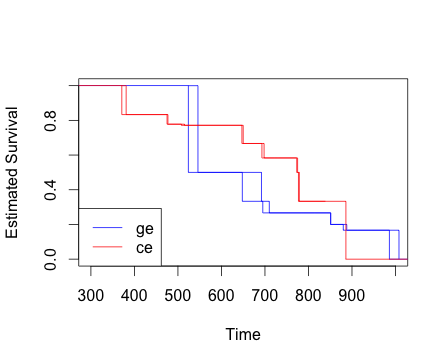
\includegraphics{MICE_NPMLES.png}}
  \caption[MICE NPMLE]{NPMLE's for both groups in miceData} 
  \label{figure:MICE}
  \end{figure}

  Looking at figure \ref{figure:MICE}, we can see a unique feature about the NPMLE for 
  interval censored data. That is, there are \emph{two} lines used to represent
  the survival curve. This is because with interval censored data, the NPMLE
  is not always unique (in fact, it usually is not); any curve that lies between
  the two lines has the same likelihood. For example, any curve that lies between
  the two blues lines in figure \ref{figure:MICE} maximizes the likelihood 
  associated with \texttt{"ge"} group of mice. 

  Formal statistical tests using the NPMLE are not currently supported by 
{\bf icenReg}. We recommend using the {\bf interval} package for this. 

  As noted earlier, \texttt{ICNPMLE} can be used to fit the univariate
  or bivariate NPMLE. However, there currently are no methods for plotting
  or testing on these fits. Because of this, we will not cover the use of this
  function here. The curious user is welcome to view \texttt{?ICNPMLE}.

  \section{Semi-parametric models}

  Semi-parametric models can be fit with \texttt{ic\_sp} function. This function
  follows standard regression syntax. As an example, we will fit the 
  \texttt{essIncData} dataset. In this dataset, we have income from the European
  Social Survey, which includes income reported up to an interval (to preserve
  the identity of the subjects). Within each country, the intervals are disjoint,
  but between countries there is penty of overlap. 
  
  We fit the model below. Note that this may be time consuming, as the semi-parametric
  model is somewhat computationally intense and we are 
  taking \texttt{bs\_samples} bootstrap samples of the estimator. 
  
  \begin{verbatim}
  fit_ph <- ic_sp(cbind(inc_l, inc_u) ~ cntry + eduLevel,
      bs_samples = 500, data = essIncData)
      
  fit_po <- ic_sp(cbind(inc_l, inc_u) ~ cntry + eduLevel,
      bs_samples = 500, model = "po", data = essIncData)
  \end{verbatim}

  The first model by default fits a Cox-PH model, while the second fits
  a proportional odds model. We can look at the results using either the
  \texttt{summary} function, or just directly looking at the results
  (what is displayed is the same). 
  
  \begin{verbatim}
> fit_po

Model:  Proportional Odds 
Baseline:  semi-parametric 
Call: ic_sp(formula = cbind(inc_l, inc_u) ~ cntry + eduLevel, 
    data = essIncData, model = "po", bs_samples = 500)

                 Estimate Exp(Est) Std.Error z-value p
cntryPoland        2.6190   13.730   0.05724  45.760 0
cntryRussia        0.7940    2.212   0.05450  14.570 0
cntrySlovakia      0.6351    1.887   0.06766   9.387 0
eduLevel[12,16)    1.0050    2.732   0.05186  19.380 0
eduLevel[16,Inf)   1.8550    6.390   0.05875  31.570 0

final llk =  -12483.03 
Iterations =  18 
Bootstrap Samples =  500 
  \end{verbatim}

  For the semi-parametric models, bootstrap samples are used
  for inference on the regression parameters. The reason for this 
  is that as far as we know, the limiting distribution of the 
  baseline distribution is currently not characterized. In fact, to our 
  knowledge, even using the bootstrap error estimates for the baseline
  distribution is not valid. Because the regression parameters cannot
  be seperated in the likelihood function, using the negative inverse of the Hessian
  for the regression standard errors is not generally valid. However, it has been
  shown that using the bootstrap for inference \emph{on the regression parameters}
  leads to valid inference. 

  We can use these fits to create plots as well. The \texttt{plot} function 
  will plot the estimated survival curves or CDF for subjects with the set of 
  covariates provided in the \texttt{newdata} argument. If \texttt{newdata}
  is left equal to \texttt{NULL}, the baseline survival function will be plotted. 
  
  If we wanted to plot the estimated CDF  
  for an individual with between
  zero and 12 years of school from Russia against the estimated CDF for an
  individual from Bulgaria with 16+ years of school, this can be done with 
  
  \begin{verbatim}
  newdata <- data.frame(cntry = c("Russia", "Bulgaria"),
    eduLevel = c("[0,12)", "[16,Inf)") )
    
  rownames(newdata) <- c("Russian/Low Ed", 
    "Bulgarian/High Ed")

  plot(fit_po, newdata, fun = "cdf", 
    lgdLocation = "bottomright", xlab = "income in Euros")
  \end{verbatim}
  
  \begin{figure}
  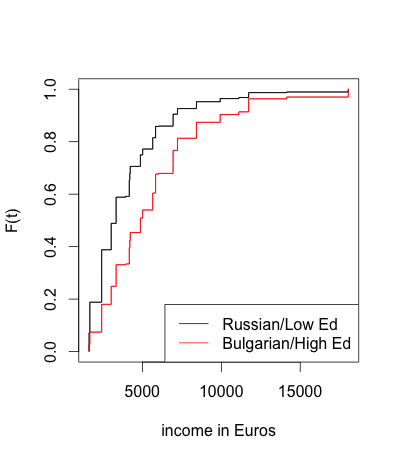
\includegraphics{essIncCDF.png}
  \label{figure:RusvBulg}
  \end{figure}
  
  \section{Parametric Models}
  
  We can fit parametric models in {\bf icenReg} using the \texttt{ic\_par} function. 
  The syntax is essentially the same as above, except that the user needs to specify
  \texttt{dist}, the parametric family that the baseline distribution belongs to. 
  The current choices are \texttt{"exponential", "weibull"} (default), 
  \texttt{"gamma", "lnorm", "loglogistic"} and \texttt{"generalgamma"} (generalized 
  gamma distribution). The user must also select \texttt{model = "ph"} or \texttt{"po"}, 
  just as in the semi-parametric model. 
  
  It is not necessary to specify \texttt{bs\_samples} for parametric models, as 
  inference is done using the asymptotic normality of the estimators. Fitting a 
  parametric model is typically faster than the semi-parametric model, even if 
  no bootstrap samples are taken for the semi-parametric model. This is because the 
  fully-parametric model is of lower dimensional space without constraints. 
  
  Suppose we wanted to fit a proportional odds model to the \texttt{essIncData} data 
  with a log-normal distribution. This could be fit by
  
  \begin{verbatim}
  fit_po_ln <- ic_par(cbind(inc_l, inc_u) ~ eduLevel + cntry,
    data = essIncData, model = "po", dist = "lnorm")
  \end{verbatim}
  
  We can examine the regression coefficients in the same way as with the semi-parametric model.
  
  \begin{verbatim}
> fit_po_ln

Model:  Proportional Odds 
Baseline:  lnorm 
Call: ic_par(formula = cbind(inc_l, inc_u) ~ eduLevel + cntry, 
    data = essIncData, model = "po", dist = "lnorm")

                 Estimate  Exp(Est) Std.Error z-value p
mu                 8.3780 4350.0000  0.007509 1116.00 0
log_s             -0.4880    0.6138  0.010240  -47.65 0
eduLevel[12,16)    1.0150    2.7590  0.048860   20.77 0
eduLevel[16,Inf)   1.8550    6.3910  0.064710   28.66 0
cntryPoland        2.5860   13.2800  0.066930   38.64 0
cntryRussia        0.8493    2.3380  0.055360   15.34 0
cntrySlovakia      0.7928    2.2090  0.062990   12.58 0

final llk =  -14413.81 
Iterations =  11 
  \end{verbatim}
  
  We can also examine the survival/cdf plots in the same way. 
  
  \begin{verbatim}
   plot(fit_po_ln, newdata, fun = "cdf", 
    lgdLocation = "bottomright", xlab = "income in Euros")
  \end{verbatim}

  \begin{figure}
  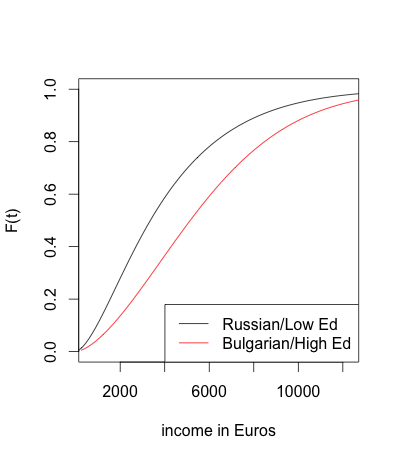
\includegraphics{essIncCDF_par.png}
  \label{figure:RusvBulg_par}
  \end{figure}

\chapter{Inspecting model fit}

  \section{Examining Baseline Distribution}
  
  Althought the semi-parametric model is more flexible, and thus more robust to unusual 
  baseline distributions, there are many reasons one may decide to use a parametric model
  instead. One reasons is that, as stated earlier, we are not aware of any general distributional
  theory regarding the baseline distribution, outside of the univariate case with case I 
  interval censored data. Even in this case, the estimator is highly inefficient, observing
  convergence rates of $n^{1/3}$ instead of the more standard $n^{1/2}$. Because of this,
  making inference about values that directly require the baseline distribution, such
  as creating a confindence interval for the median for subjects with a given set of 
  covariates, cannot be done with the semi-parametric model. Secondly, we have found that
  when it comes to cross-validation (to be described shortly), 
  we often found the semi-parametric estimator
  to be overly optimistic for some loss functions in comparison with a parametric model. 
  
  However, even if a parametric model is used for final inference, the semi-parametric model
  is still useful for assessing model fit. This is especially important for interval censored
  data, as we do not have the option of examining typical residuals or histograms as we would
  if the outcome was uncensored. {\bf icenReg} has the function \texttt{diag\_baseline} that plots 
  several choices of parametric baseline distributions against the semi-parametric estimate. 
  If the parametric distribution shows no systematic deviations from the semi-parametric
  fit, this implies the choice of parametric family may do a reason job of describing the 
  underlying distribution. If there are clear deviations, this model should not be trusted. 
  
  To use \texttt{diag\_baseline}, you must provide either a fitted model, or a formula,
  data and model. You then select the parametric families that you would like plotted 
  against the non-parametric estimate (default is to fit all available).
  As an example, suppose we wanted to 
  examine the different parametric fits for the \texttt{essIncData} dataset. This could 
  be done with 
  
  \begin{verbatim}
  diag_baseline(cbind(inc_l, inc_u) ~
    eduLevel + cntry,
    model = "po",
    data = essIncData,
    lgdLocation = "topright")
  \end{verbatim}
  
  Alternatively, using the fits from earlier, we can just call
  
  \begin{verbatim}
  diag_baseline(fit_po,lgdLocation = "topright")
  \end{verbatim}
  
  \begin{figure}
  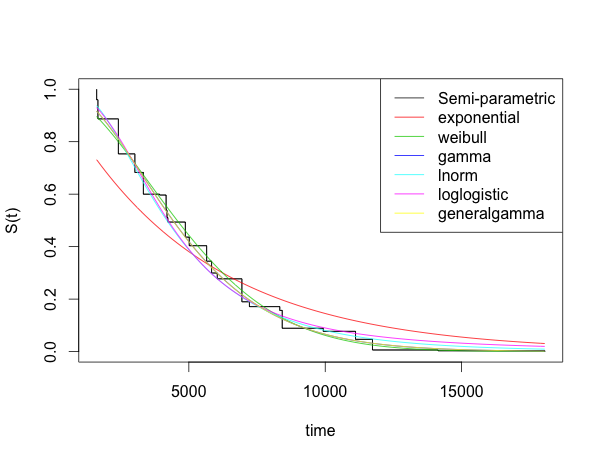
\includegraphics{diagBaseline.png}
  \label{figure:diagBase}
  \end{figure}
  
  Visual diagnostics are always subjective, but in this case we 
  definitively know that the exponential fit is not appropriate 
  and we believe the log-normal baseline is most appropriate 
  for the proporitonal odds model. 
  \section{Examining Covariate Effect}
  
  Although semi-parametric models do not make assumptions about the 
  parametric family of the baseline distribution, both fully-parametric 
  and semi-parametric models make assumptions about the form of the 
  covariate effect, akin to the link function in generalized linear
  models. 
  
  A rule of thumb for identifying gross violations of proportional
  hazards is to check if the Kaplan Meier curves cross; if they do,
  and this cross appears not purely by chance, the proportional 
  hazards assumption seems inappropriate. 
  
  This can naturally extend to the case of interval censored data 
  by replacing the Kaplan Meier curves with the NPMLE. Also, this
  informal test can be generalized to the proportional odds model;
  the proportional odds assumption also implies that survival curves
  that differ only by a constant factor of the odds of survival 
  should not cross. 
  
  Another method of assessing involves transforming your 
  survival estimates such that if the assumptions are met,
  the difference in transformed survival will be constant. 
  For the proportional hazards model, this is the complementary 
  log-log tranformation (i.e. $\log (-\log(s) )$). For the 
  proportional odds model, this is the logit transformation
  (i.e. $\log(s/(1-s))$ ).
  
  Plotting these functions can be done automatically in 
 {\bf icenReg} using the \texttt{diag\_covar} function. The
 basic flow is that function takes in the fit, divides the data
 up on a covariate of interest. If it is categorical, it simply
 breaks up by category, if it is numeric, it attempts to find
 break point to evenly split up the data. Then, for each subset of 
 the data, it fits the corresponding semi-parametric model and
 plots the transformation of the baseline distribution. 
 
 To demonstrate, suppose we wanted to assess whether the Cox-PH
 or proportional odds model was more appropriate for the 
 \texttt{essIncData}. This could be done by 
 
 \begin{verbatim}
 diag_covar(fit_po, lgdLocation = "topright")
 diag_covar(fit_ph, lgdLocation = "topright")
 \end{verbatim}

  \begin{figure}
  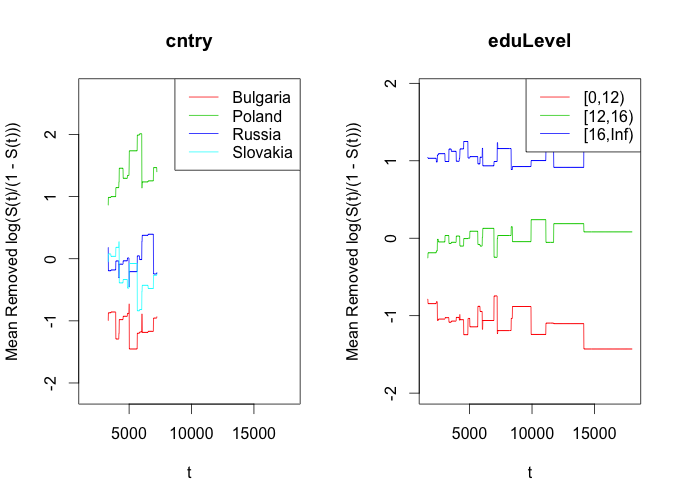
\includegraphics{diagCovarPO.png}
  \end{figure}
  
  \begin{figure}
  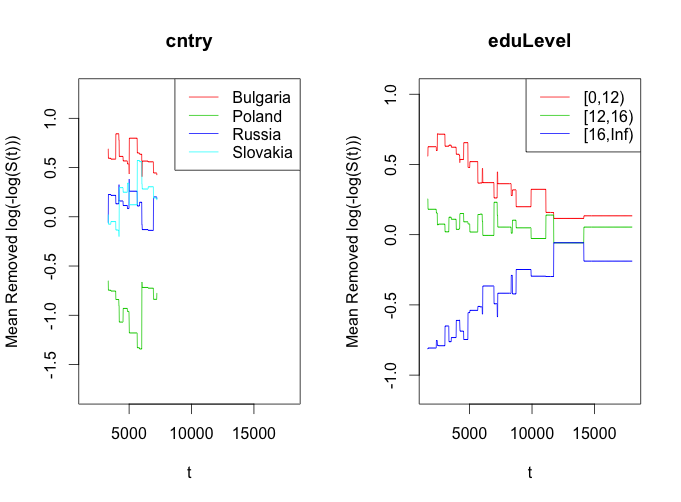
\includegraphics{diagCovarPH.png}
  \end{figure}

  We see that especially for eduLevel, the porportional odds
  seems much more appropriate (the difference between 
  transformed values seems more constant). This agrees
  with the fact that the likelihood is almost 100 greater
  for the proportional odds model than Cox-PH. 
  
  Note that the plots for cntry are very limited. This is 
  because the mean trend is removed from the plots. However,
  since the cdf for the semi-parametric model for the 
  Bulgaria subset of the data is defined as exactly 1 around 
  10,000, the mean of the transformation is not defined. 
  
  We can replot the transformation, without the mean removed,
  by the following call:
  
  \begin{verbatim}
  diag_covar(fit_po, yType = "transform",
    lgdLocation = "topright")
  \end{verbatim}

  \begin{figure}
  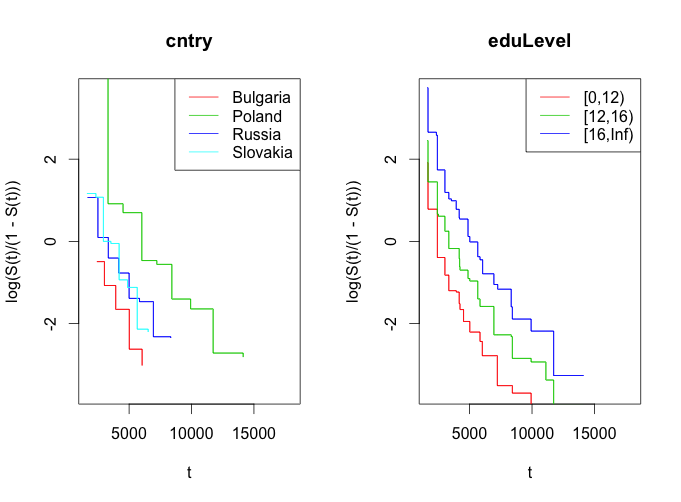
\includegraphics{transformPlot.png}
  \label{figure:tranformKeepMean}
  \end{figure}


\section{Imputed Cross Validation}

  Cross validation is a popular method for evaluating how well a model will perform 
  on new data. In general, 
  the idea is simple enough: to get an estimate of some loss function on
  out of sample data for a given model, we split the data into training
  and validation datasets. The training dataset is used to fit the model
  (without touching the validation data). Then an estimate of the out of
  sample error can be generated by predicting the response in the validation
  dataset and directly computing the loss function. In K-fold cross validation,
  K disjoint subsets of the data are used as validation datasets and the process
  is repeated K-times. 
  
  For censored data, this generic recipe is not so simple. In particular, if 
  a value in the validation set is censored, there is typically no direct
  method for calculating the contribution to the loss function 
  associated with this observation. 
  
  One method to deal with censoring that has appeared in the literature is to calculate
  likelihood over the validation data set. As an alternative, we offer an imputation
  based approach. To calculate the
  average loss function, we take several imputations (or samples) of the 
  interval censored data condtional on the covariates \emph{and censoring interval}
  (i.e. the distribution is truncated such that the imputation will fall inside the
  given censoring interval). The average loss across all imputations is then taken
  as the evaluated loss. 
  
  To impute the data, we first take a sample of the posterior parameters and conditional
  on the parameters and censoring interval, we sample the censored values. An important
  note is that {\bf icenReg} does \emph{not} sample the baseline parameters, but only
  the regression parameters for the semi-parametric model. This means that the 
  uncertainity in the baseline parameteris is ignored. 
  For the fully parametric model, both the regression and
  baseline parameters are sampled.

  For the prediction, the median value conditional on the parameter estimates is used. 
  This is \emph{not} neccesarily the estimate that minimizes the loss function, but it 
  is generally a reasonable estimate. 
  
  Cross validation can be done with {\bf icenReg}'s \texttt{icenReg\_cv} function. 
  This takes a regression model (either from \texttt{ic\_par} or \texttt{ic\_sp}), and a
  loss function to be calculated.
  CAUTION: When using cross-validation on an \texttt{ic\_sp} fit, the total number of 
  models fit will be \texttt{fold} (default = 10) x \texttt{bs\_samples}. This can get
  very expensive very quickly!
  
  The default loss function is \texttt{abs\_inv}, which is 
  defined as 
  
  \begin{verbatim}
  abs_inv <- function(pred, t_val) {
    mean(abs(1/(pred + 1) - 1/(t_val + 1)))
  }
  \end{verbatim}

  Although we believe this to be a reasonable loss function for survival data
  (heavy penalizes for missing subjects that are at high risk, does not heavily 
  penalizing for not being precise with low-risk subjects as long as they are identified as low risk),
  this function is not the final say in loss functions. 
  A user can write their own loss function, which should take in arguments
  \texttt{pred} and \texttt{t\_val}, where \texttt{pred} is the predicted
  value and \texttt{t\_val} is the true response value. 
  
  Imputed cross validation can then be used as such:
  
  \begin{verbatim}
  icenReg_cv(fit = fit_po, loss_fun = abs_inv)
  \end{verbatim}
  
  
  \section{Appendix}
  
  Both the bootstrap and cross validation statistics can be extremely computationally
  expensive, yet also are both embarrassingly parallel problems. As such, they are 
  written take advantage of multiple cores via the {\bf doParallel} package. 
  Below is demonstrated how to run the bootstrap and cross validation using 
  four cores. 
  
  
  \begin{verbatim}
  library(doParallel)
  myCluster <- makeCluster(4, type = 'FORK')
  registerDoParallel(myCluster)
  fit <- ic_sp(cbind(inc_l, inc_u) ~ eduLevel + cntry,
            data = essIncData, model = "po",
            bs_samples = 50, useMCores = TRUE)
            
  par_fit <- ic_par(cbind(inc_l, inc_u) ~ eduLevel + cntry,
                dist = "lnorm", model = "po",
                data = essIncData)
                

  cv_error <- icenReg_cv(par_fit)
  #Fit a parametric model because it is much faster;
  #does not need to fit bootstrap samples for each
  #training set
  
  stopCluster(myCluster)
  \end{verbatim}
  
  
\end{document}
